% ===========================================================================
%  Slides de Conferência (ANPEC) --- Enchentes RS 2024
%  Tema: Metropolis | Idioma: Português | 22 slides | 15–20 min
%  Compile: xelatex (3 passes + bibtex)
% ===========================================================================

\documentclass[11pt, aspectratio=169]{beamer}

% ── Tema ────────────────────────────────────────────────────────────────────
\usetheme[
  block        = fill,
  progressbar  = frametitle,
  numbering    = fraction,
]{metropolis}

% ── Fontes (XeLaTeX) ─────────────────────────────────────────────────────────
\usepackage{ifxetex}
\ifxetex
  \usepackage{fontspec}
  \IfFontExistsTF{Fira Sans}{%
    \setsansfont[BoldFont={Fira Sans SemiBold}]{Fira Sans}%
  }{%
    \setsansfont{Arial}%
  }
  \IfFontExistsTF{Fira Mono}{%
    \setmonofont{Fira Mono}%
  }{}
\fi
\usefonttheme[onlymath]{serif}

% ── Idioma ───────────────────────────────────────────────────────────────────
\usepackage[brazil]{babel}
\usepackage[utf8]{inputenc}
\usepackage[T1]{fontenc}

% ── Pacotes ──────────────────────────────────────────────────────────────────
\usepackage{booktabs}
\usepackage{graphicx}
\usepackage{amsmath, amssymb}
\usepackage{xcolor}
\usepackage{microtype}
\usepackage{csquotes}
\usepackage[alf, abnt-etal-list=0]{abntex2cite}

% ── Figuras ──────────────────────────────────────────────────────────────────
\graphicspath{
  {./}
  {../Artigos/SDID/Resultados/SDID completo pool completo 6 municipios/}
  {../Artigos/SDID/Resultados/SDID triangulacao DiD SC SDID/}
  {../Artigos/SDID/Resultados/SDID event study twfe/}
  {../Artigos/SDID/Resultados/SDID heterogeneidade dano/}
  {../Artigos/SDID/Resultados/SDID sensibilidade pool/}
}

% ── Cores ────────────────────────────────────────────────────────────────────
\definecolor{mblue}{HTML}{1F4E79}
\definecolor{mred}{HTML}{C0392B}
\definecolor{mgray}{HTML}{7F8C8D}
\definecolor{mgreen}{HTML}{1A7A4A}

\setbeamercolor{frametitle}{bg=mblue}
\setbeamercolor{progress bar}{fg=mred}
\setbeamercolor{alerted text}{fg=mred}

% ── Comandos auxiliares ───────────────────────────────────────────────────────
\newcommand{\destaque}[1]{\textcolor{mred}{\textbf{#1}}}
\newcommand{\positivo}[1]{\textcolor{mgreen}{\textbf{#1}}}

% ── Metadados ────────────────────────────────────────────────────────────────
\title{Emprego Formal e Desastres Climáticos}
\subtitle{Evidências Causais das Enchentes de 2024 no Rio Grande do Sul}
\author{Arthur P. Donato \and A. T. G. Fiorentin \and G. S. Teixeira \and M. V. B. Santos \and T. M. Brito}
\institute{PPGE -- Universidade Federal do Rio Grande (FURG)}
\date{2025}

% ===========================================================================
\begin{document}

% ---------------------------------------------------------------------------
% 1 --- TÍTULO
% ---------------------------------------------------------------------------
\maketitle

% ---------------------------------------------------------------------------
% 2 --- MOTIVAÇÃO: A CATÁSTROFE
% ---------------------------------------------------------------------------
\begin{frame}[shrink=8]{Motivação: O Maior Desastre Climático do RS}

\begin{columns}[T]
\begin{column}{0.55\textwidth}
  \textbf{Abril--Maio/2024:}
  \begin{itemize}
    \item \destaque{478 municípios} afetados ($>90\%$ do estado)
    \item \destaque{2,4 milhões} de pessoas atingidas
    \item 388 mil desalojados; 178 óbitos
    \item Municípios mais atingidos: \destaque{50--82\%} da população
  \end{itemize}

  \medskip
  \textbf{Mercado de trabalho formal:}
  \begin{itemize}
    \item IPEA: \destaque{84--92\%} dos postos formais afetados nos municípios mais atingidos
  \end{itemize}
\end{column}
\begin{column}{0.42\textwidth}
  \begin{alertblock}{Choque sem precedente}
    Como mensurar causalmente o efeito sobre o emprego formal quando as áreas afetadas não são amostra aleatória?
  \end{alertblock}
\end{column}
\end{columns}

\end{frame}

% ---------------------------------------------------------------------------
% 3 --- PERGUNTA E CONTRIBUIÇÕES
% ---------------------------------------------------------------------------
\begin{frame}[shrink=20]{Pergunta e Contribuições}

\textbf{Pergunta:} Qual o efeito causal das enchentes de 2024 sobre as \emph{admissões} em emprego formal nos municípios gaúchos mais atingidos?

\medskip

\begin{block}{Contribuições}
  \begin{enumerate}
    \item \textbf{Empírica:} Primeiras estimativas SDiD para inundações no Brasil, desagregadas por município
    \item \textbf{Metodológica:} Triangulação TWFE-DiD $\times$ SC $\times$ SDiD sobre o mesmo painel, janela e pool
    \item \textbf{Substantiva:} Identifica o canal produtivo (firmas + viário) como principal mecanismo de transmissão ao emprego formal
  \end{enumerate}
\end{block}

\end{frame}

% ---------------------------------------------------------------------------
% 4 --- POR QUE ADMISSÕES?
% ---------------------------------------------------------------------------
\begin{frame}{Por que Admissões Formais, e Não o Estoque?}

\textbf{Achado-chave da literatura próxima} \cite{teixeira2024}:

\medskip

\begin{columns}[T]
\begin{column}{0.48\textwidth}
  \begin{block}{Desligamentos}
    Variação estatisticamente \textbf{nula} nos municípios atingidos

    \smallskip
    Razão: rigidez da legislação trabalhista brasileira
  \end{block}
\end{column}
\begin{column}{0.48\textwidth}
  \begin{alertblock}{Admissões}
    \textbf{Retração significante e persistente}

    \smallskip
    O ajuste operou pela \emph{margem de entrada}: bloqueio de novas contratações
  \end{alertblock}
\end{column}
\end{columns}

\medskip
\textbf{Consequência:} O fluxo de admissões é o indicador privilegiado da recuperação pós-desastre. É exatamente esse componente que este estudo estima.

\end{frame}

% ---------------------------------------------------------------------------
% 5 --- DESAFIO DE IDENTIFICAÇÃO
% ---------------------------------------------------------------------------
\begin{frame}{Desafio de Identificação}

\textbf{Problema:} municípios inundáveis \emph{não} são amostra aleatória --- concentram-se em áreas de risco com características correlacionadas com renda e capacidade institucional.

\smallskip
\textbf{Comparações simples} $\Rightarrow$ capturam diferenças pré-existentes, não o efeito causal.

\smallskip
\begin{columns}[T]
\begin{column}{0.48\textwidth}
  \begin{block}{Exogeneidade do timing}
    A intensidade das chuvas de maio/2024 não era previsível com antecedência suficiente para antecipação contratual \cite{elsner2024}
  \end{block}
\end{column}
\begin{column}{0.48\textwidth}
  \begin{block}{SDiD + pool de doadores}
    Controla heterogeneidade de nível e trajetórias divergentes sem exigir tendências paralelas em nível \cite{arkhangelsky2021}
  \end{block}
\end{column}
\end{columns}

\end{frame}

% ---------------------------------------------------------------------------
% 6 --- DADOS
% ---------------------------------------------------------------------------
\begin{frame}{Dados}

\begin{columns}[T]
\begin{column}{0.55\textwidth}
  \textbf{Variável dependente}
  \begin{itemize}
    \item Admissões formais por mil habitantes/mês
    \item Fonte: CAGED (microdados mensais)
    \item Janela: jan./2021--mar./2025 (51 meses)
    \item \textbf{40 meses pré} + \textbf{11 meses pós}
  \end{itemize}

  \medskip
  \small Início em jan./2021: após consolidação do Novo CAGED (eSocial) e fase aguda da pandemia.
\end{column}
\begin{column}{0.42\textwidth}
  \textbf{Design}
  \begin{itemize}
    \item \textbf{6 tratados}: $>50\%$ da população atingida \cite{teixeira2024}
    \item \textbf{193 doadores}: $\leq 0{,}5\%$ atingidos (zona \textit{donut})
    \item Covariáveis: emprego pré-2021, porte, setor dominante, IDESE
  \end{itemize}
\end{column}
\end{columns}

\end{frame}

% ---------------------------------------------------------------------------
% 7 --- OS 6 MUNICÍPIOS
% ---------------------------------------------------------------------------
\begin{frame}{Os 6 Municípios Tratados}

\begin{center}
\footnotesize
\begin{tabular}{lrrl}
\toprule
Município & Pop.\ (2022) & \% Atingida & Perfil \\
\midrule
Eldorado do Sul & 39.559 & \destaque{82,2\%} & Urbano-industrial (RM-PoA) \\
Muçum           &  4.601 & 79,1\%            & Agroindústria (Vale Taquari) \\
Roca Sales      & 10.418 & 54,5\%            & Agroindústria (Vale Taquari) \\
Travesseiro     &  2.152 & 51,0\%            & Agropecuária \\
Arambaré        &  4.112 & 51,9\%            & Serviços/pesca (Lagoa dos Patos) \\
Igrejinha       & 32.808 & 50,9\%            & Industrial (calçados/couro) \\
\bottomrule
\end{tabular}
\end{center}

\medskip
\footnotesize
Critério de inclusão: $>50\%$ da pop.\ atingida \cite{teixeira2024}.
Critério de exclusão do pool: $\leq 0{,}5\%$ atingidos (zona \textit{donut} para mitigar transbordamentos).

\end{frame}

% ---------------------------------------------------------------------------
% 8 --- ESTRATÉGIA: SDiD
% ---------------------------------------------------------------------------
\begin{frame}[shrink=10]{Estratégia de Identificação: SDiD}

\textbf{Intuição:} combina o melhor do DiD e do Controle Sintético \cite{arkhangelsky2021}

\smallskip

O SDiD estima dois conjuntos de pesos antes da regressão principal:

\begin{columns}[T]
\begin{column}{0.48\textwidth}
  \begin{block}{Pesos de unidade $\hat{\omega}_i$ (à la SC)}
    Equilibram trajetórias pré-tratamento entre tratados e doadores --- sem exigir convex hull
  \end{block}
\end{column}
\begin{column}{0.48\textwidth}
  \begin{block}{Pesos de tempo $\hat{\lambda}_t$ (novidade)}
    Concentram peso nos períodos pré-tratamento mais informativos sobre o contrafactual
  \end{block}
\end{column}
\end{columns}

\smallskip
\textbf{Estimador:}
\[
(\hat{\tau}^{\text{sdid}},\ldots) = \arg\min_{\tau,\mu,\alpha,\beta}
\sum_{i,t}\!\left(Y_{it} - \mu - \alpha_i - \beta_t - \tau D_{it}\right)^{\!2}\!\hat{\omega}_i\,\hat{\lambda}_t
\]

\textbf{Dupla robustez:} consistente se os pesos de unidade \emph{ou} os de tempo forem corretamente especificados \cite{arkhangelsky2021}

\end{frame}

% ---------------------------------------------------------------------------
% 9 --- VERIFICAÇÃO: EVENT STUDY
% ---------------------------------------------------------------------------
\begin{frame}{Verificação: Pré-Tendências (Event Study TWFE)}

\begin{center}
  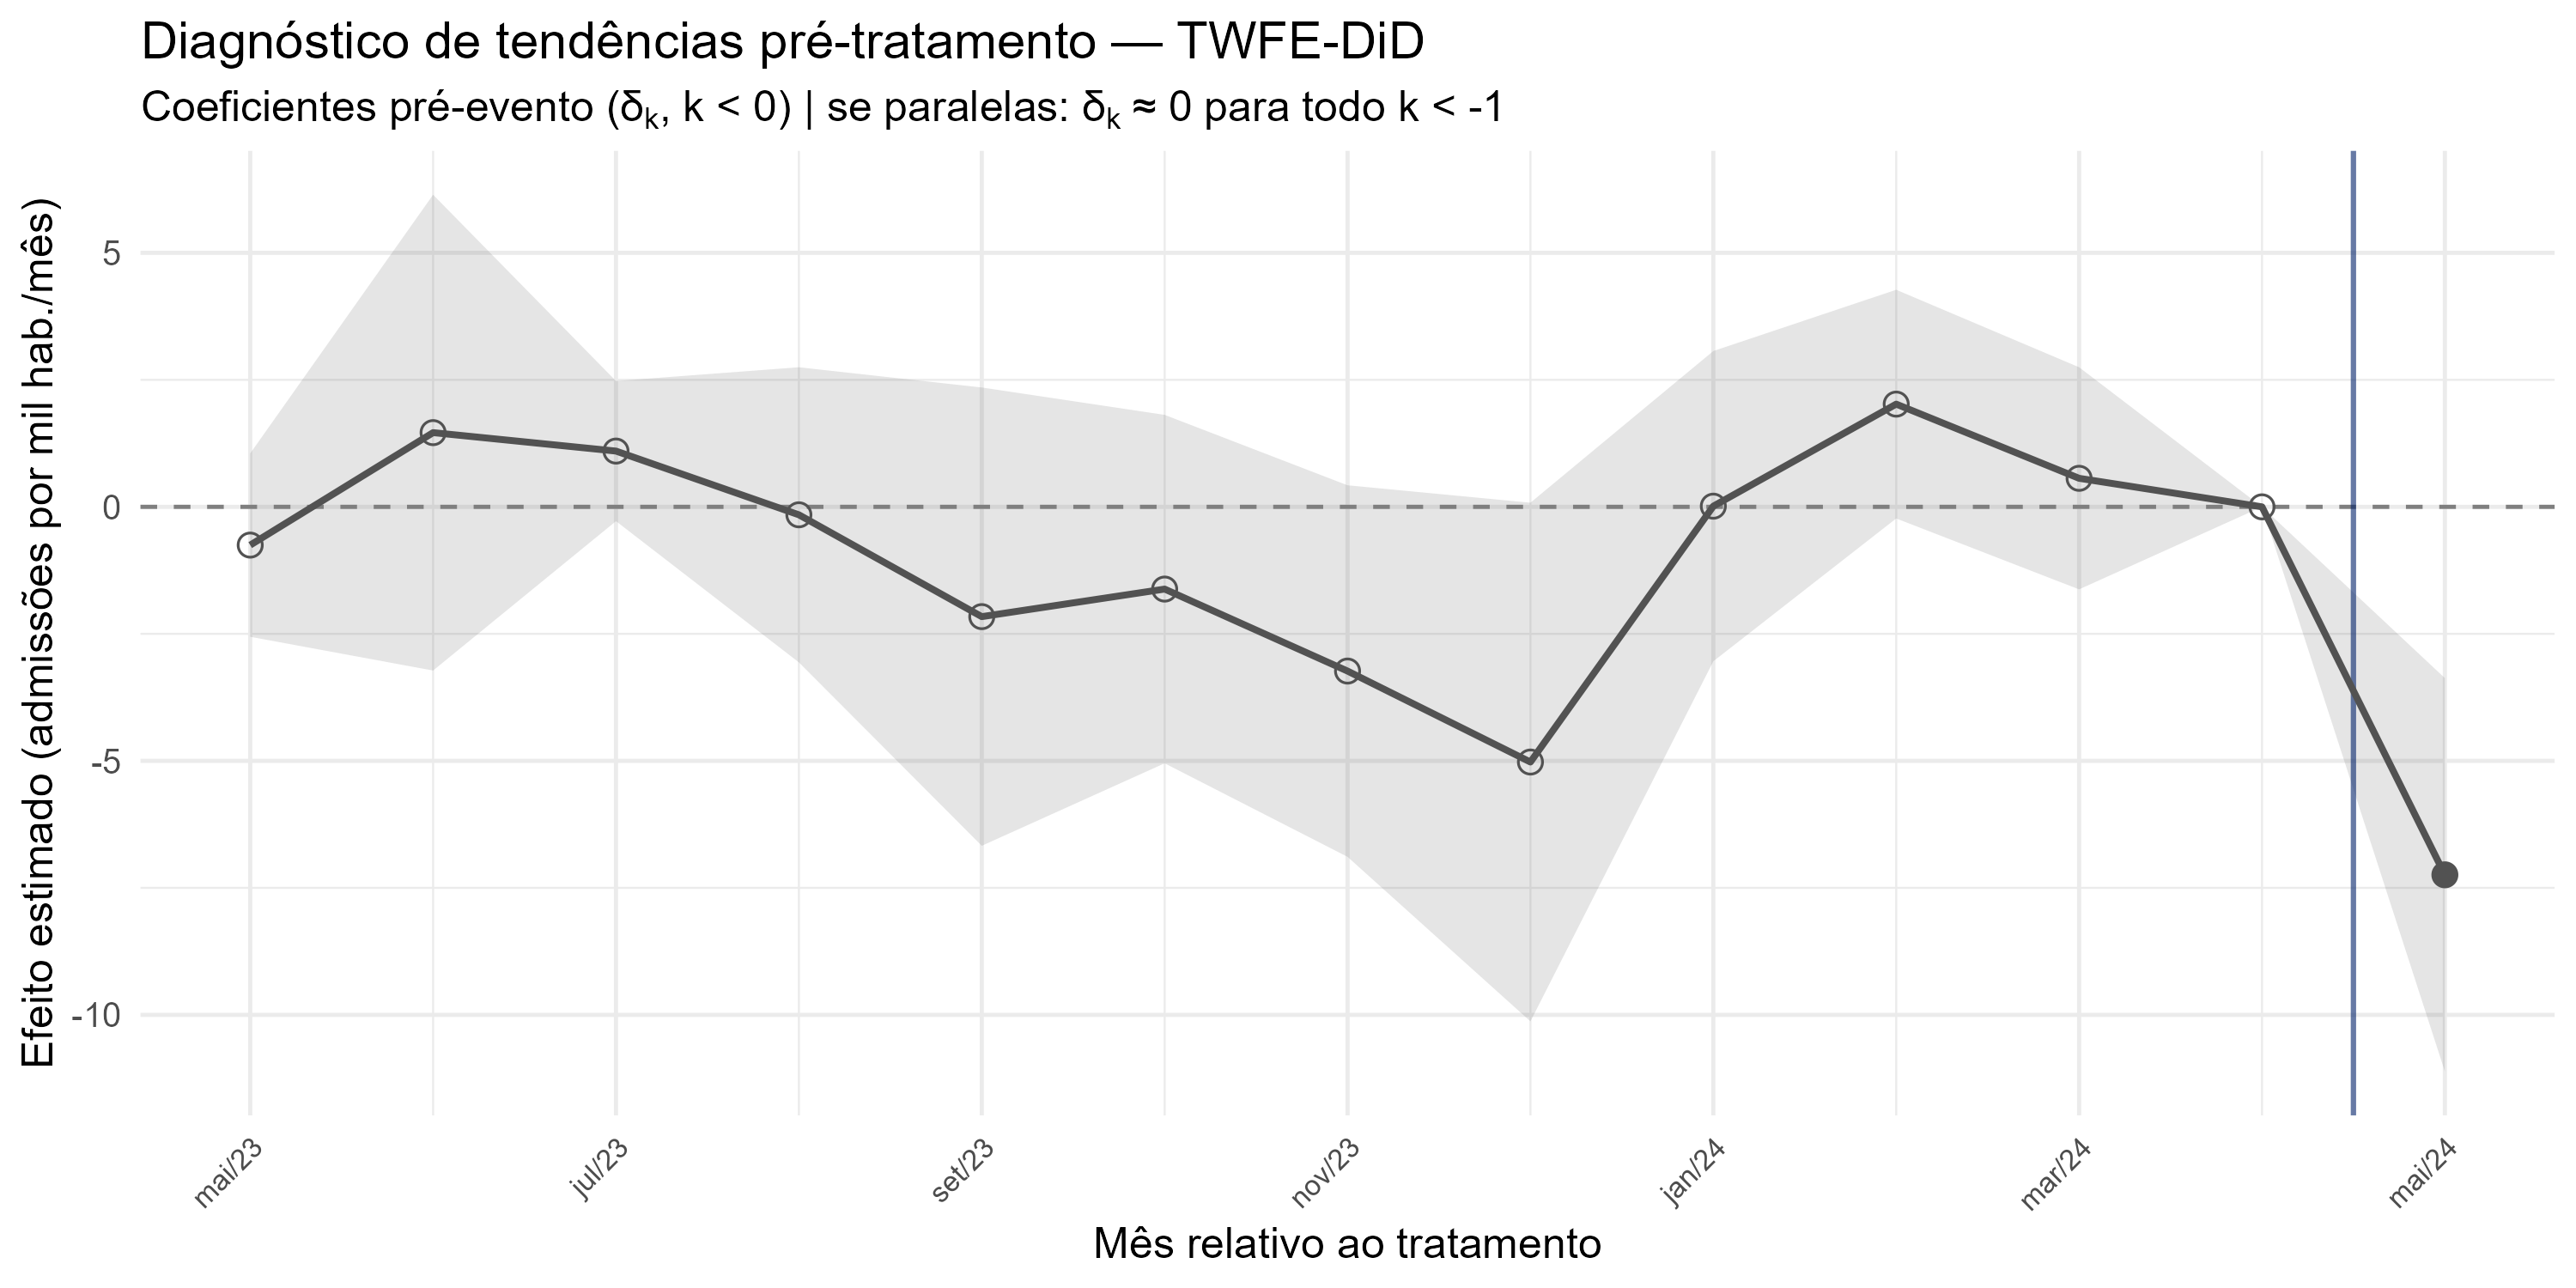
\includegraphics[height=0.65\textheight]{event_study_pre_zoom.png}
\end{center}

\footnotesize
Coeficientes pré-tratamento não significantes a 5\% $\Rightarrow$ suporte à hipótese de tendências paralelas.
Linha vertical: mai./2024 (tratamento).

\end{frame}

% ---------------------------------------------------------------------------
% 10 --- RESULTADO PRINCIPAL: ATT
% ---------------------------------------------------------------------------
\begin{frame}{Resultado Principal: ATT (SDiD, pool completo)}

\begin{center}
\footnotesize
\begin{tabular}{lrrrl}
\toprule
Município & ATT & IC\,95\% & $p$ & Classificação \\
\midrule
Eldorado do Sul & \destaque{$-3{,}72$} & $[-7{,}04;\,-0{,}52]$ & 0,041 & Efeito robusto \\
Muçum           & \destaque{$-5{,}08$} & $[-7{,}74;\,-2{,}17]$ & 0,016 & Provável$^{\dagger}$ \\
Roca Sales      & \destaque{$-3{,}72$} & $[-6{,}37;\,-0{,}58]$ & 0,036 & Efeito robusto \\
Travesseiro     & \destaque{$-3{,}73$} & $[-7{,}11;\,-0{,}63]$ & 0,036 & Efeito robusto \\
Arambaré        & $-0{,}06$            & $[-3{,}10;\,+3{,}03]$ & 0,943 & Sem efeito \\
Igrejinha       & $-1{,}34$            & $[-4{,}40;\,+1{,}78]$ & 0,207 & Sem efeito \\
\bottomrule
\end{tabular}
\end{center}

\footnotesize
ATT em admissões por mil hab./mês. IC\,95\% por permutação direta (193 doadores).
$^{\dagger}$ RMSPE\,pré $>5{,}0$: inferência parcial.

\medskip
\textbf{Padrão:} nos municípios robustos, ATT converge em torno de \destaque{$-3{,}72$} adm./mil hab./mês.

\end{frame}

% ---------------------------------------------------------------------------
% 11 --- TRAJETÓRIAS SDiD
% ---------------------------------------------------------------------------
\begin{frame}{Trajetórias SDiD: Tratado vs.\ Controle Sintético}

\begin{center}
  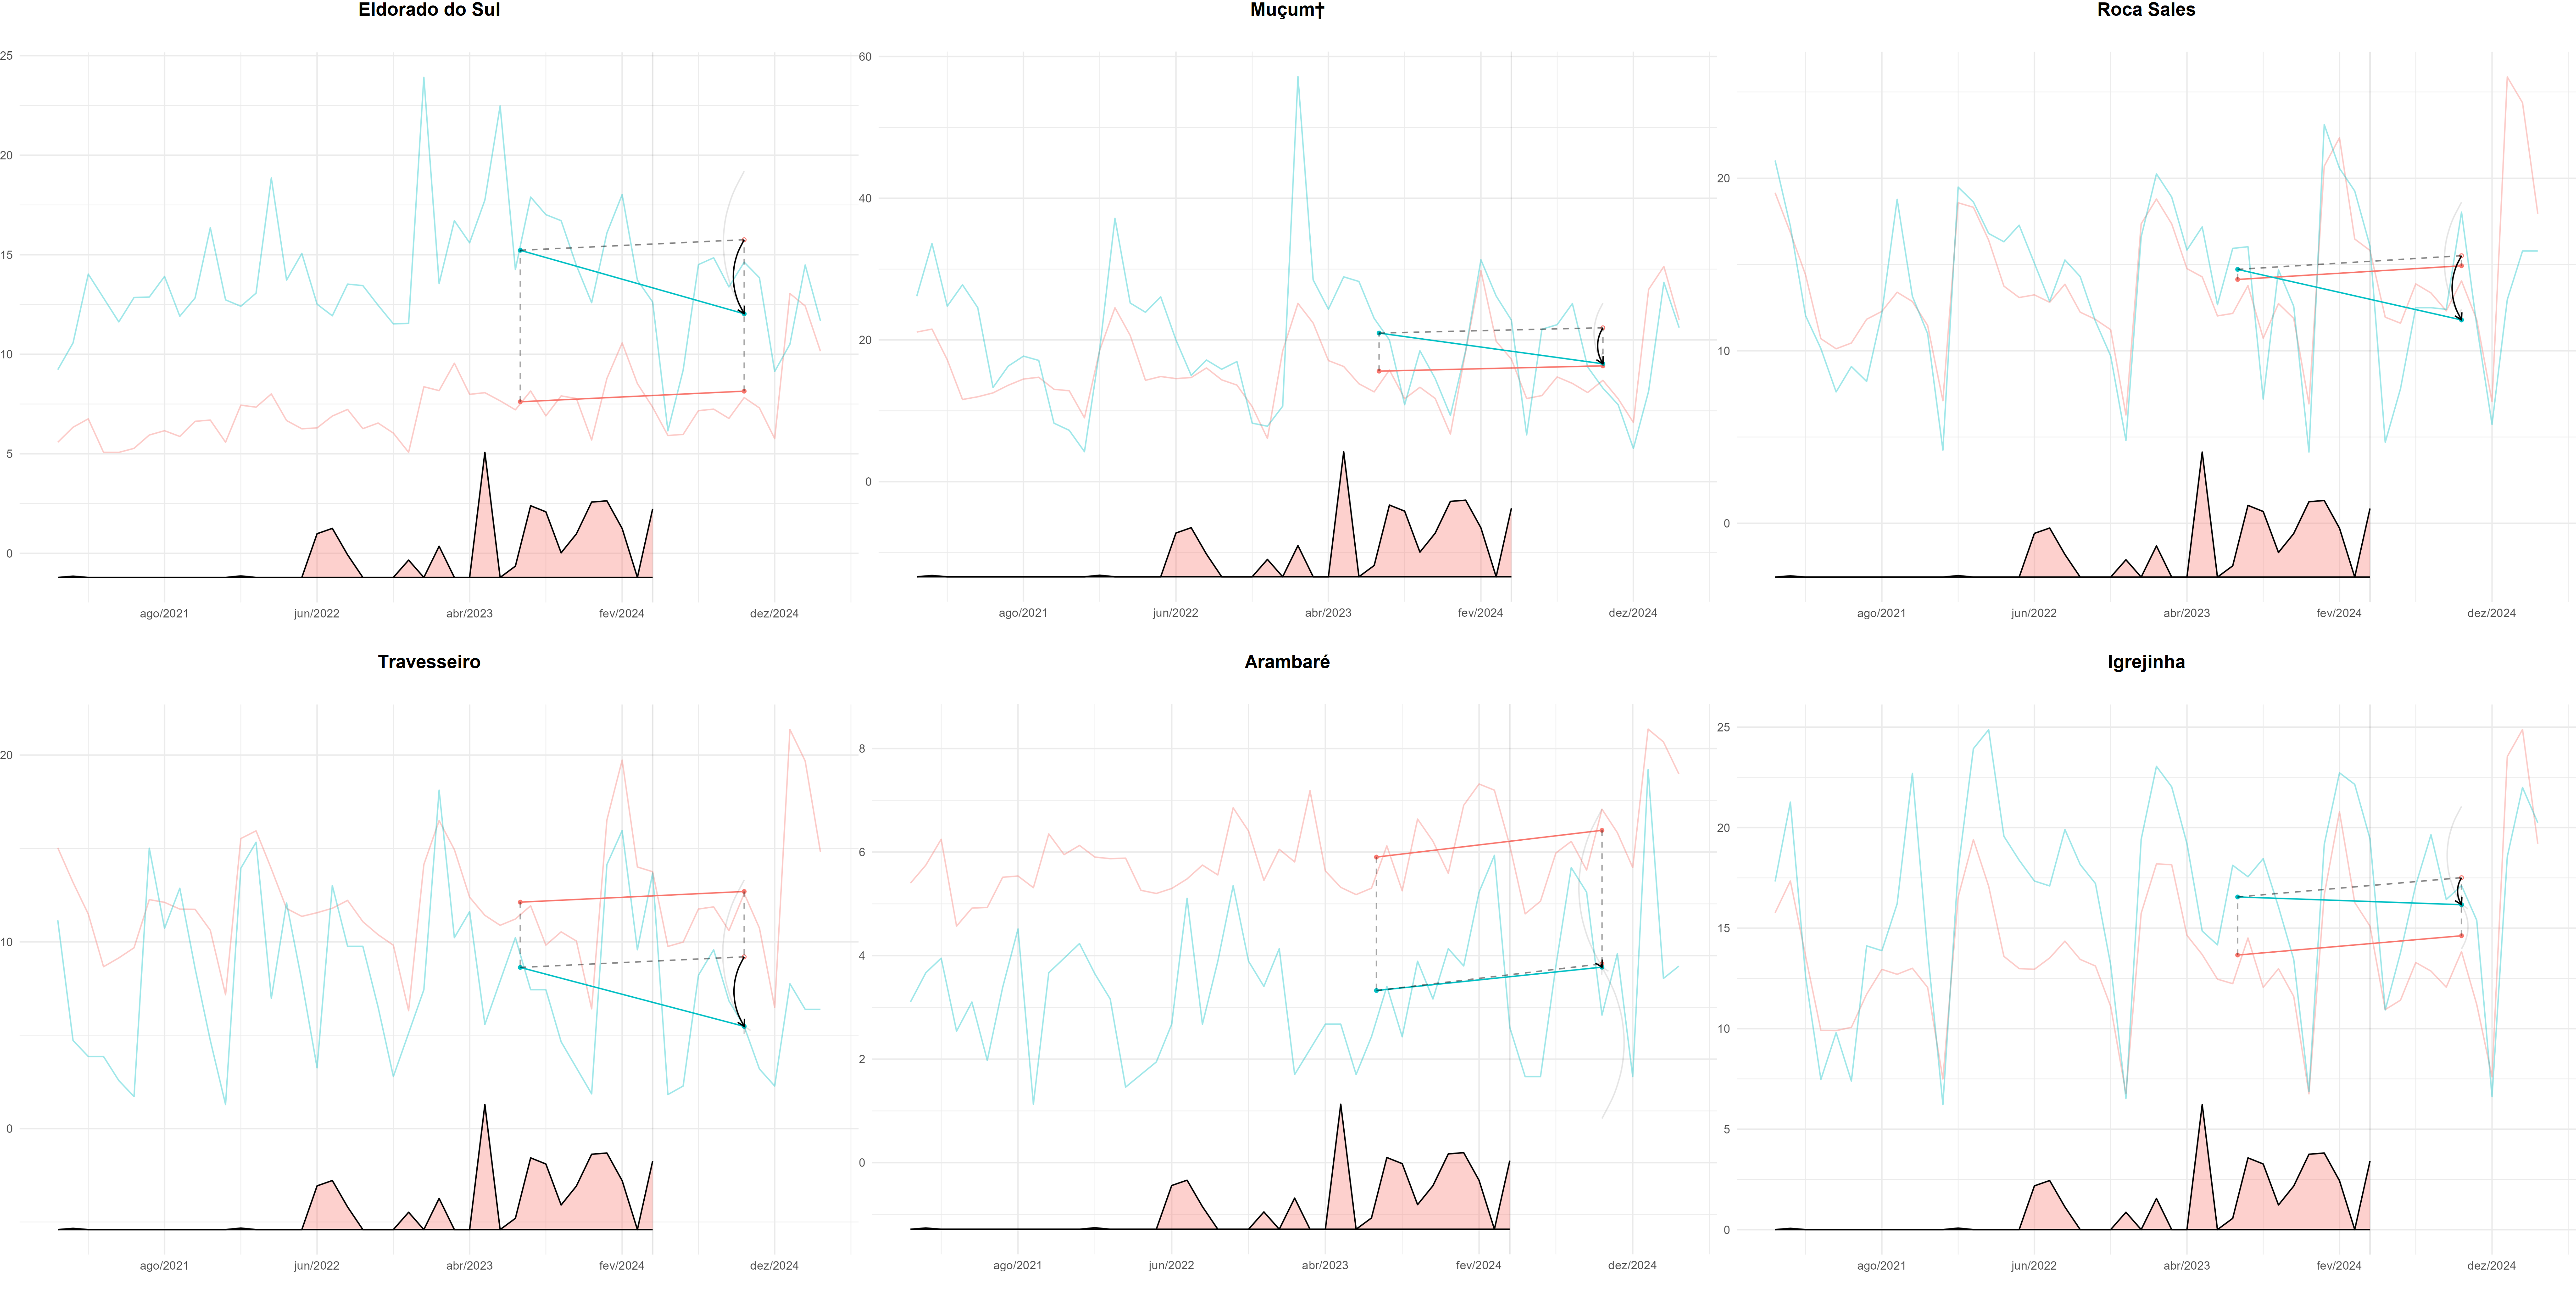
\includegraphics[width=\textwidth, height=0.68\textheight, keepaspectratio]{figura1_trajetorias_todos.png}
\end{center}

\footnotesize
\textbf{Azul:} unidade tratada. \textbf{Laranja:} controle sintético SDiD. Linha vertical: mai./2024.
Área sombreada: pesos temporais $\hat{\lambda}_t$ (concentrados nos meses pré-desastre).

\end{frame}

% ---------------------------------------------------------------------------
% 12 --- INFERÊNCIA: PLACEBOS
% ---------------------------------------------------------------------------
\begin{frame}{Inferência por Permutação: Forest Plot}

\begin{center}
  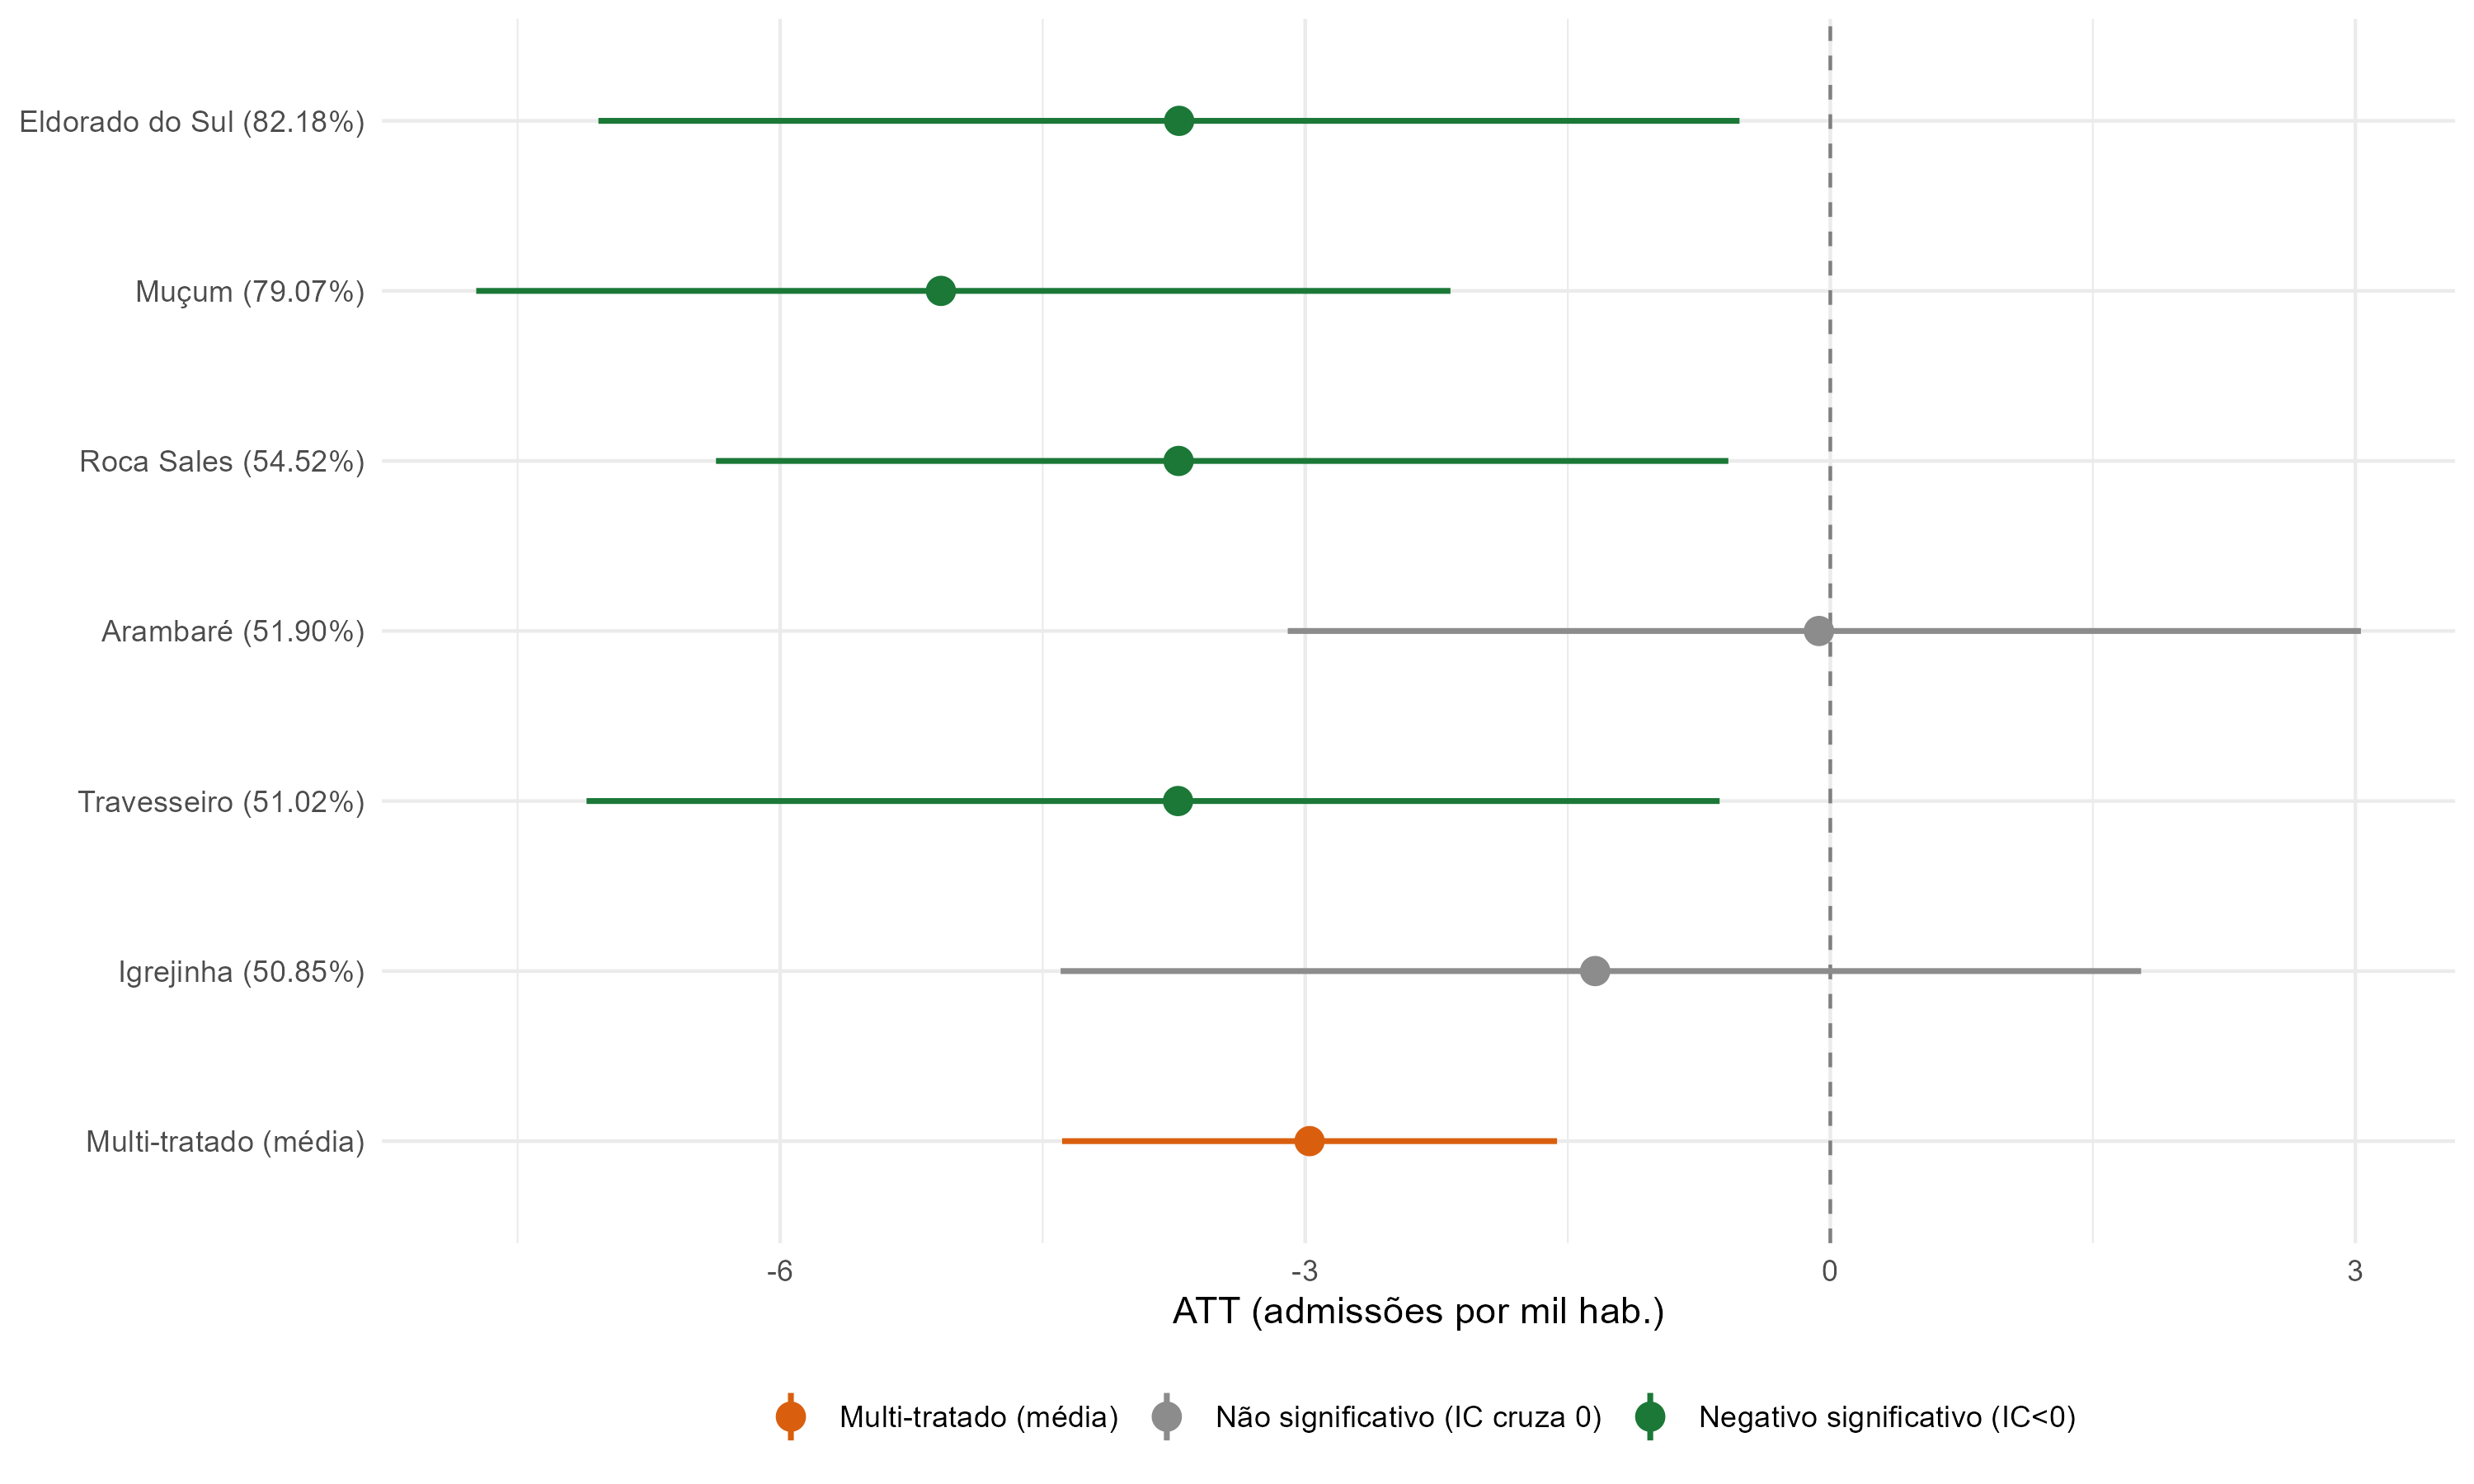
\includegraphics[height=0.67\textheight]{forest_plot_completo.png}
\end{center}

\footnotesize
Cada ponto: ATT estimado; barras: IC\,95\% por permutação (193 doadores).
\destaque{Círculos cheios}: IC exclui zero (efeito robusto). Círculos vazios: sem efeito.

\end{frame}

% ---------------------------------------------------------------------------
% 13 --- TRIANGULAÇÃO
% ---------------------------------------------------------------------------
\begin{frame}{Triangulação: TWFE-DiD, SC e SDiD}

\begin{center}
  \includegraphics[height=0.67\textheight]{triangulacao_forest.png}
\end{center}

\footnotesize
Três estimadores, mesmo painel, janela e pool.
\textbf{Convergência} de sinal e magnitude nos 4 municípios com efeito.
Amplitude máxima entre estimadores: $\leq 1{,}00$ adm./mil (exceto Muçum).

\end{frame}

% ---------------------------------------------------------------------------
% 14 --- EFEITO ACUMULADO (TABELA)
% ---------------------------------------------------------------------------
\begin{frame}{Efeito Acumulado: Empregos Formais Não Gerados}

\begin{center}
\footnotesize
\begin{tabular}{lrrl}
\toprule
Município & Pop.\ (2022) & Efeito Acumulado & IC\,95\% \\
\midrule
Eldorado do Sul & 39.559 & \destaque{$-1.619$} & $[-3.141;\,-97]$ \\
Roca Sales      & 10.418 & $-427$ & $[-828;\,-26]$ \\
Muçum           &  4.601 & $-257$ & $[-434;\,-80]$ \\
Travesseiro     &  2.152 & $-88$  & $[-171;\,-5]$ \\
Igrejinha       & 32.808 & $-485$ & $[-1.747;\,+777]$ \\
Arambaré        &  4.112 & $-3$   & $[-161;\,+155]$ \\
\midrule
\textbf{4 municípios robustos} & & \destaque{$>2.390$ déficit} & \\
\bottomrule
\end{tabular}
\end{center}

\smallskip
\footnotesize
Acumulado mai./2024--mar./2025 (11 meses). Admissões \emph{não geradas} em razão do choque.\\
Efeito sobre desligamentos: estimado como nulo \cite{teixeira2024}.

\end{frame}

% ---------------------------------------------------------------------------
% 15 --- DINÂMICA TEMPORAL
% ---------------------------------------------------------------------------
\begin{frame}{Dinâmica Temporal: Curva de Efeito Acumulado}

\vfill
\begin{center}
  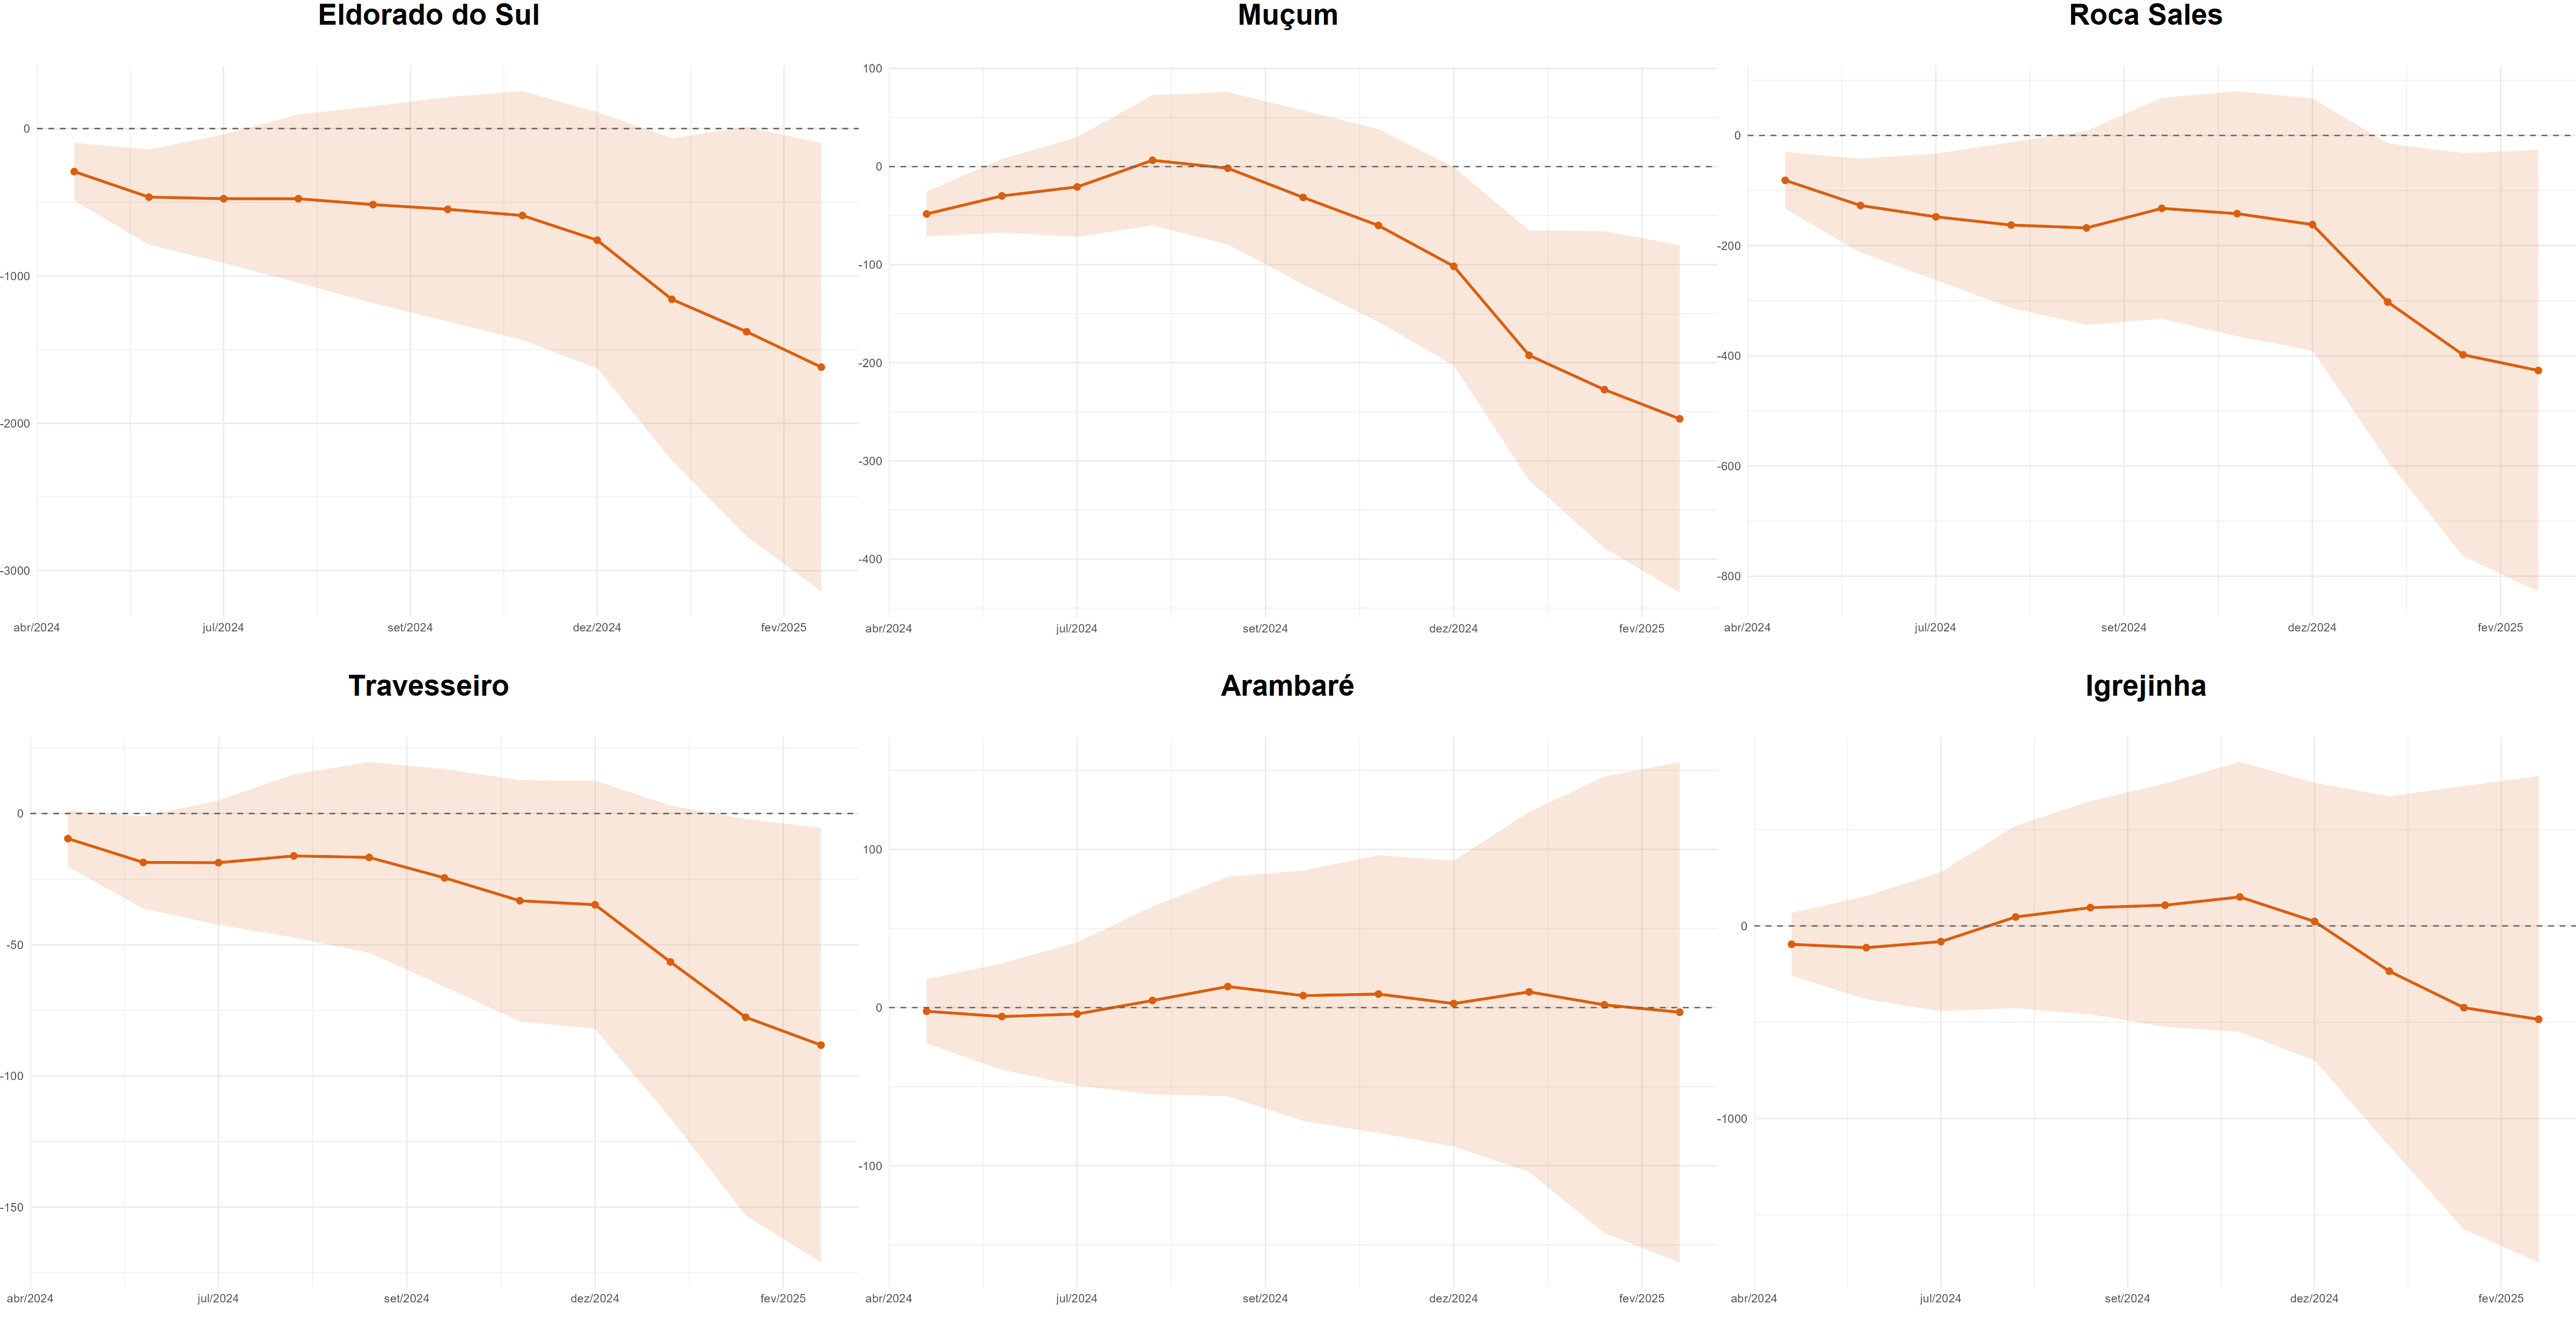
\includegraphics[width=\textwidth, height=0.68\textheight, keepaspectratio]{figura11_efeito_acumulado_todos.png}
\end{center}

\footnotesize
Padrão em ``W'': choque (mai./2024) $\to$ retomada parcial (jun.--nov./2024) $\to$ segundo pico (jan./2025).\\
Consistente com danos persistentes à infraestrutura de transporte \cite{xiao2014}.
\vfill

\end{frame}

% ---------------------------------------------------------------------------
% 16 --- HETEROGENEIDADE: CANAIS
% ---------------------------------------------------------------------------
\begin{frame}{Heterogeneidade: Quais Canais Explicam o Efeito?}

\textbf{Motivação:} Arambaré e Igrejinha ($>50\%$ pop.\ atingida) --- \emph{sem efeito detectável} no emprego formal.

\smallskip

\begin{center}
\footnotesize
\begin{tabular}{lrrl}
\toprule
Variável de Dano & $z$ (separação) & Média ``com'' & Média ``sem'' \\
\midrule
Dano viário (\% malha)          & \destaque{1,49} & 37,3\% & 27,5\% \\
Dano a firmas (\% CNPJ)         & \destaque{1,37} & 75,6\% & 52,8\% \\
Índice produtivo relativo\,$^*$ & 1,00            & 11,3\% &  0,4\% \\
Dano residencial (\% domicílios)& 1,00            & 64,3\% & 52,5\% \\
\bottomrule
\end{tabular}
\end{center}

\footnotesize
$^*$ Índice produtivo = (\% CNPJ) $-$ (\% domicílios).
\textbf{Canal produtivo} (viário + firmas) discrimina os grupos melhor que o dano residencial isolado.

\end{frame}

% ---------------------------------------------------------------------------
% 17 --- EVIDÊNCIA: CANAIS (FIGURA)
% ---------------------------------------------------------------------------
\begin{frame}{Canais de Dano por Município}

\begin{center}
  \includegraphics[height=0.67\textheight]{dano_canais_centrais.png}
\end{center}

\footnotesize
\positivo{Verde}: municípios com efeito robusto (IC\,95\% $<0$).
\textcolor{mgray}{Cinza}: sem efeito detectável.
Fonte: MUPRS/SPGG-RS e estimativas SDiD.

\end{frame}

% ---------------------------------------------------------------------------
% 18 --- ROBUSTEZ: POOL
% ---------------------------------------------------------------------------
\begin{frame}{Robustez: Sensibilidade ao Critério do Pool Doador}

\begin{center}
  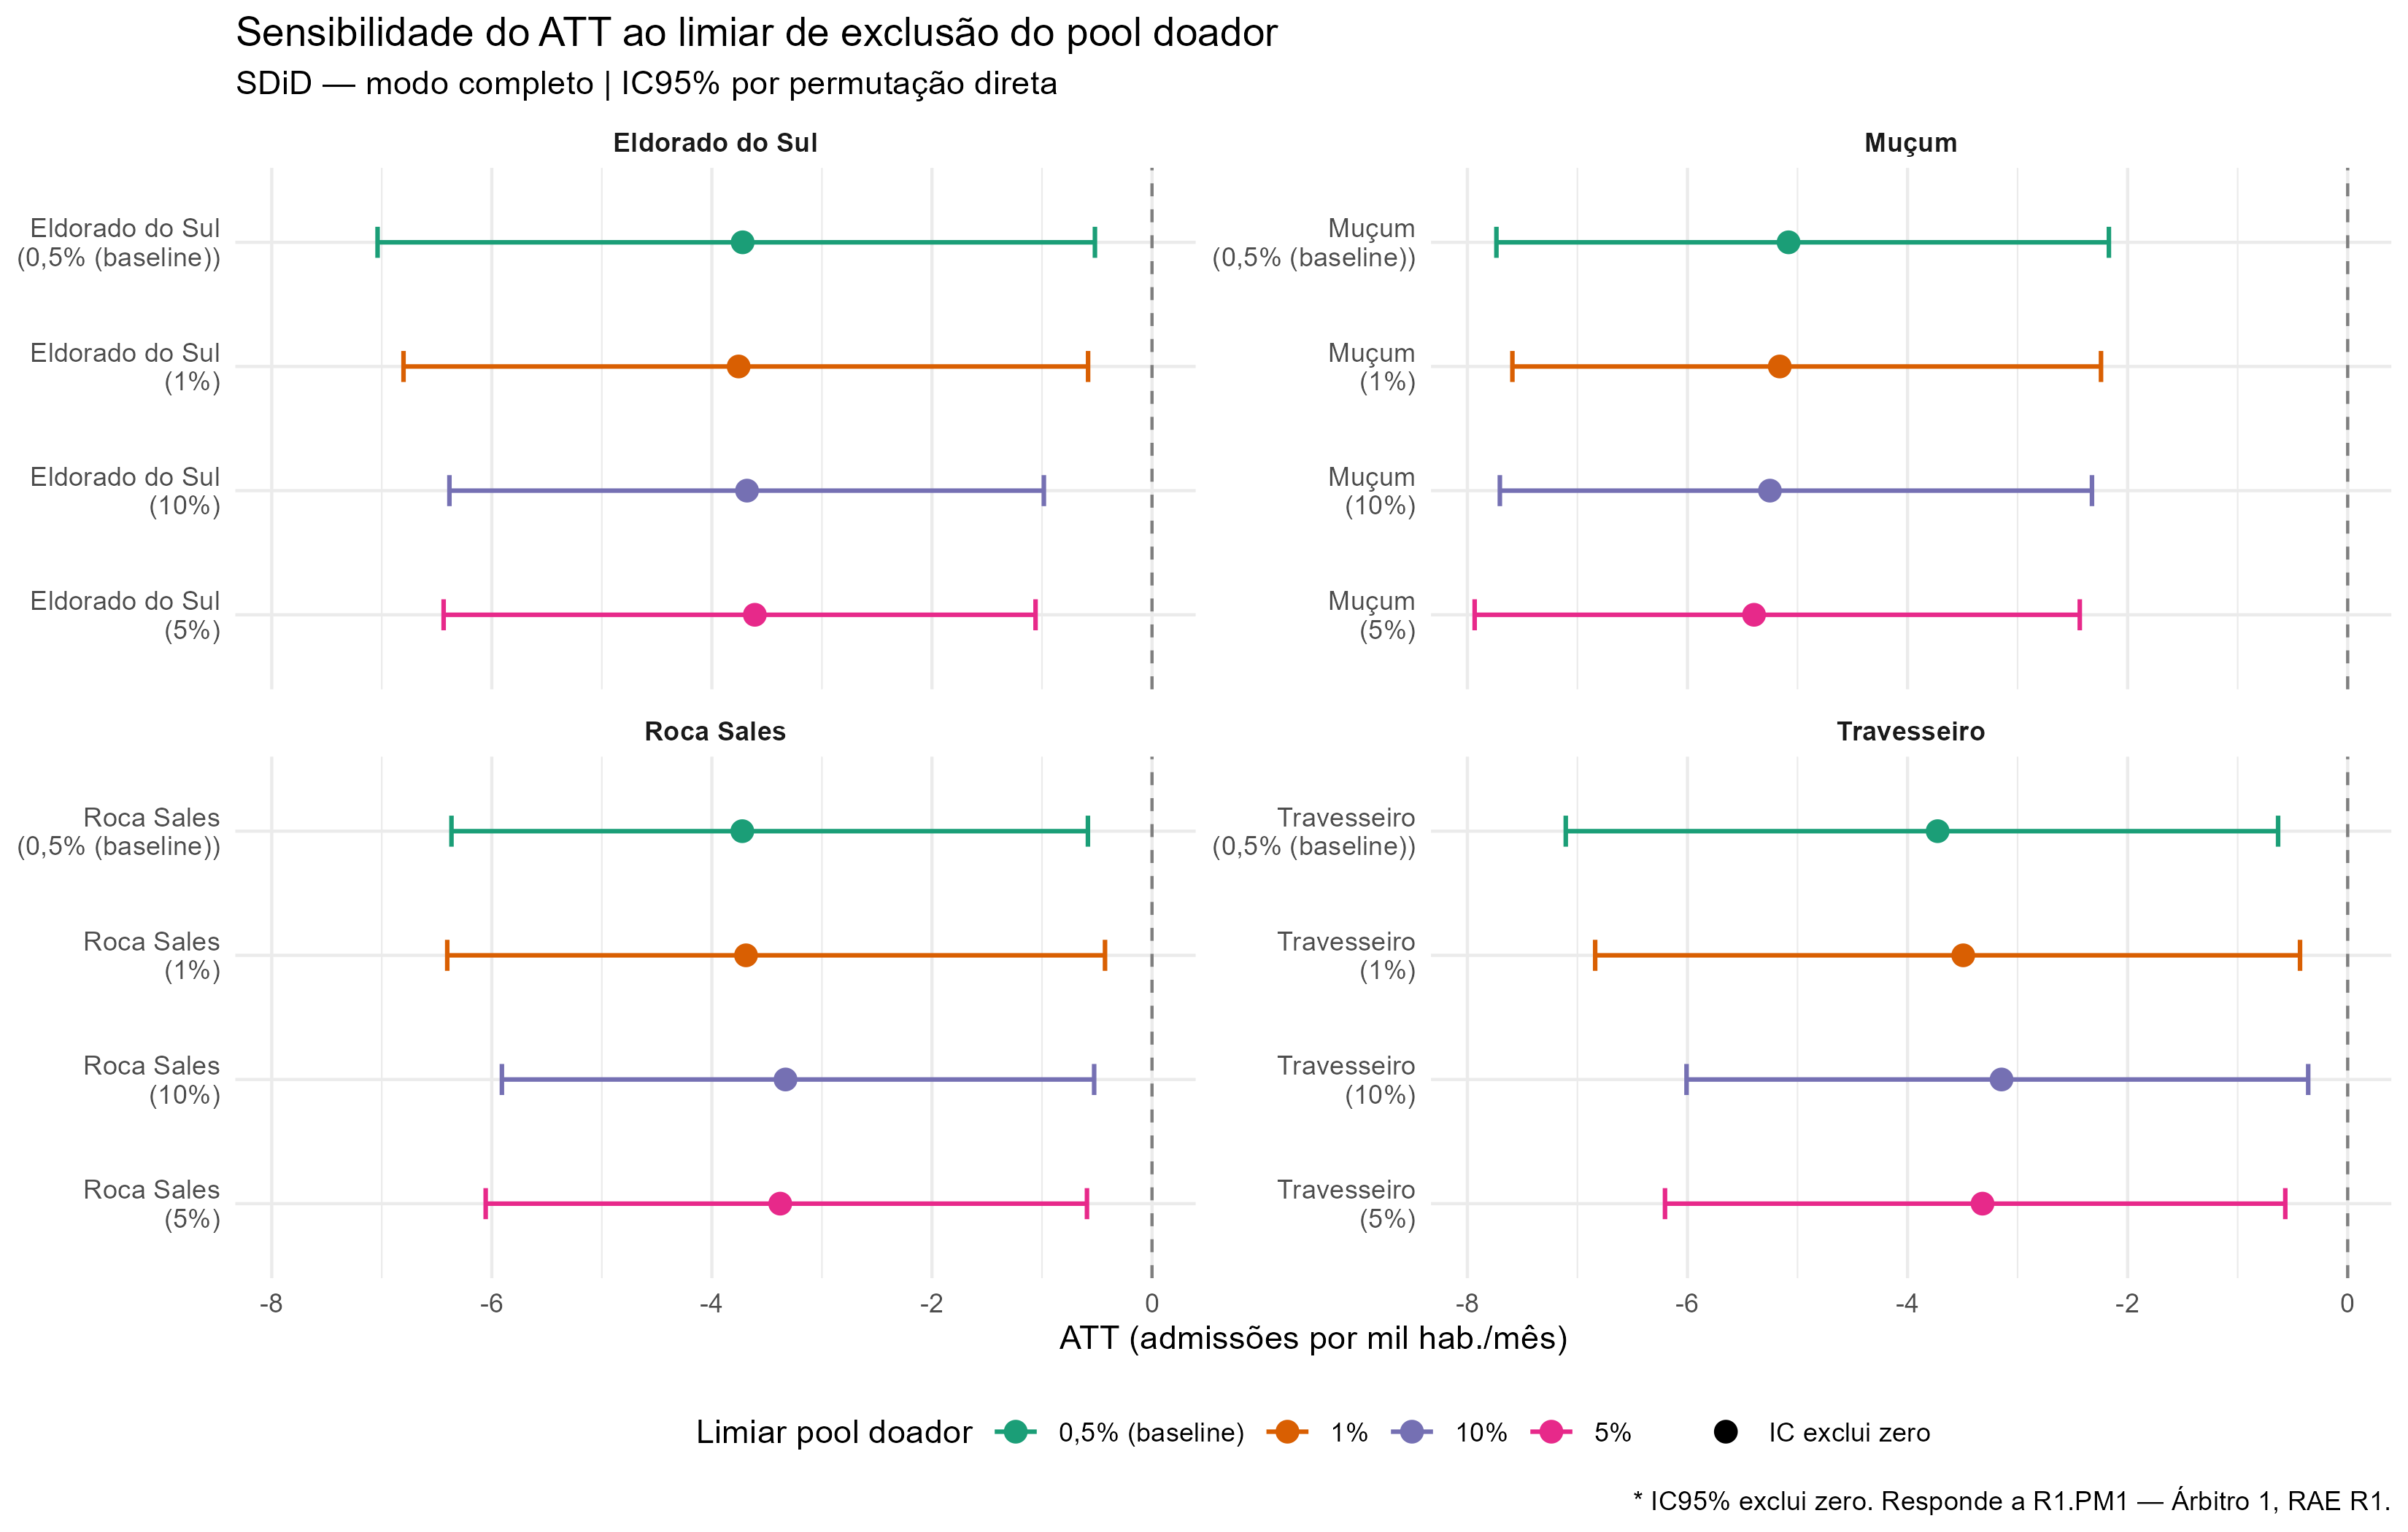
\includegraphics[height=0.67\textheight]{sensibilidade_forest.png}
\end{center}

\footnotesize
4 limiares alternativos ($N_0 = 193$ a $291$ doadores).
\textbf{16/16 ATTs negativos e significantes a 5\%}; variação máxima $<15\%$ da estimativa \textit{baseline}.

\end{frame}

% ---------------------------------------------------------------------------
% 19 --- SUMÁRIO DOS ACHADOS
% ---------------------------------------------------------------------------
\begin{frame}[shrink=5]{Sumário dos Achados}

\begin{enumerate}
  \item \textbf{Efeito robusto em 4 de 6 municípios:} ATT $\approx -3{,}7$ adm./mil hab./mês (Eldorado do Sul, Roca Sales, Travesseiro) e $-5{,}1$ (Muçum, inferência parcial)

  \item \textbf{Triangulação confirma:} TWFE-DiD, SC e SDiD convergem em sinal e magnitude --- amplitude máxima $\leq 1{,}0$ adm./mil nos três municípios de efeito estritamente robusto

  \item \textbf{Déficit acumulado} $>$ \destaque{2.390 empregos formais} ao longo de 11 meses nos municípios com efeito detectável

  \item \textbf{Heterogeneidade explicada pelo canal produtivo:} dano viário e a firmas discriminam municípios com/sem efeito melhor do que dano residencial isolado
\end{enumerate}

\end{frame}

% ---------------------------------------------------------------------------
% 20 --- IMPLICAÇÕES DE POLÍTICA
% ---------------------------------------------------------------------------
\begin{frame}{Implicações de Política Pública}

\begin{columns}[T]
\begin{column}{0.50\textwidth}
  \begin{alertblock}{Canal produtivo $>$ canal habitacional}
    Municípios com alto dano residencial mas tecido produtivo poupado (Arambaré) não exibem resposta no emprego formal
  \end{alertblock}
\end{column}
\begin{column}{0.47\textwidth}
  \begin{block}{Implicação direta}
    Pacotes de recuperação devem priorizar:
    \begin{itemize}
      \item Reconstrução de vias de escoamento
      \item Crédito emergencial às firmas
      \item Subsídios temporários à contratação
    \end{itemize}
  \end{block}
\end{column}
\end{columns}

\medskip
\footnotesize
O ajuste operou pela \emph{margem de entrada} (bloqueio de novas contratações), não por demissões. Políticas de proteção ao emprego existente eram menos necessárias neste contexto --- o ajuste já estava naturalmente limitado pela rigidez da legislação trabalhista.

\end{frame}

% ---------------------------------------------------------------------------
% 21 --- LIMITAÇÕES E AGENDA FUTURA
% ---------------------------------------------------------------------------
\begin{frame}{Limitações e Agenda Futura}

\textbf{Limitações reconhecidas:}
\begin{itemize}
  \item Emprego \emph{informal} não captado pelo CAGED --- efeito total provavelmente subestimado
  \item Análise de heterogeneidade descritiva com $n=6$ (sem inferência formal entre municípios)
  \item Janela de 11 meses pode encerrar antes da recuperação completa
\end{itemize}

\medskip
\textbf{Agenda futura:}
\begin{itemize}
  \item Ampliar janela para avaliar recuperação de longo prazo
  \item Dados do CEMPRE para identificar heterogeneidade por porte de firma
  \item Modelagem espacial (SAR-SC) para efeitos de transbordamento \cite{sakaguchi2026}
\end{itemize}

\end{frame}

% ---------------------------------------------------------------------------
% 22 --- AGRADECIMENTOS E REFERÊNCIAS
% ---------------------------------------------------------------------------
\begin{frame}{Obrigado}

\vfill
\begin{center}
{\Large \textbf{Emprego Formal e Desastres Climáticos:}}\\[6pt]
{\large Evidências Causais das Enchentes de 2024 no Rio Grande do Sul}

\medskip
\texttt{arthurdonato19@gmail.com}
\end{center}

\vfill
\hrule
\vspace{6pt}

\footnotesize
\textbf{Agradecimentos:} Este trabalho contou com apoio financeiro da \textbf{CAPES} --- Coordenação de Aperfeiçoamento de Pessoal de Nível Superior, e do \textbf{GPEA} --- Grupo de Pesquisa em Economia Azul / FURG.

\vspace{8pt}
\begin{center}
  
\includegraphics[height=1.1cm, keepaspectratio]{logo_capes.png}%
  \hspace{2.0cm}%
  
\includegraphics[height=1.1cm, keepaspectratio]{logo_gpea.png}
\end{center}
\vfill

\end{frame}

% ---------------------------------------------------------------------------
\begin{frame}[allowframebreaks]{Referências}
  \bibliography{bib_sdid}
\end{frame}

\end{document}
